\section{The harm of class imbalance corrections for risk prediction models}
	The paper argues that the class imbalance is not a pervasive problem for prediction model development. 
	First, the problem is specific to the classification accuracy measure. 
	The limitations of focusing on classification accuracy as a measure of predictive performance is well known. 
	Second, if we consider models that produce estimated probabilities of the event of interest, 
	an adjustment of the classification threshold probability can be used to ensure adequate classification performance 
	(ie, probability threshold to classify individuals as high risk does not have to be 0.5). 
	A probability threshold to select individuals for a given treatment implies certain misclassification costs and should be determined using clinical considerations. 
	If we use a probability threshold of 0.1 to classify individuals as high risk and suggest a specific treatment, 
	this means that we accept to treat up to 10 individuals in order to treat 1 individual with the event: 
	we accept up to 9 false positives, or unnecessary treatments, per true positive.
	
\subsection{Discussion}
<<<<<<< HEAD
	\begin{figure}[h]
         	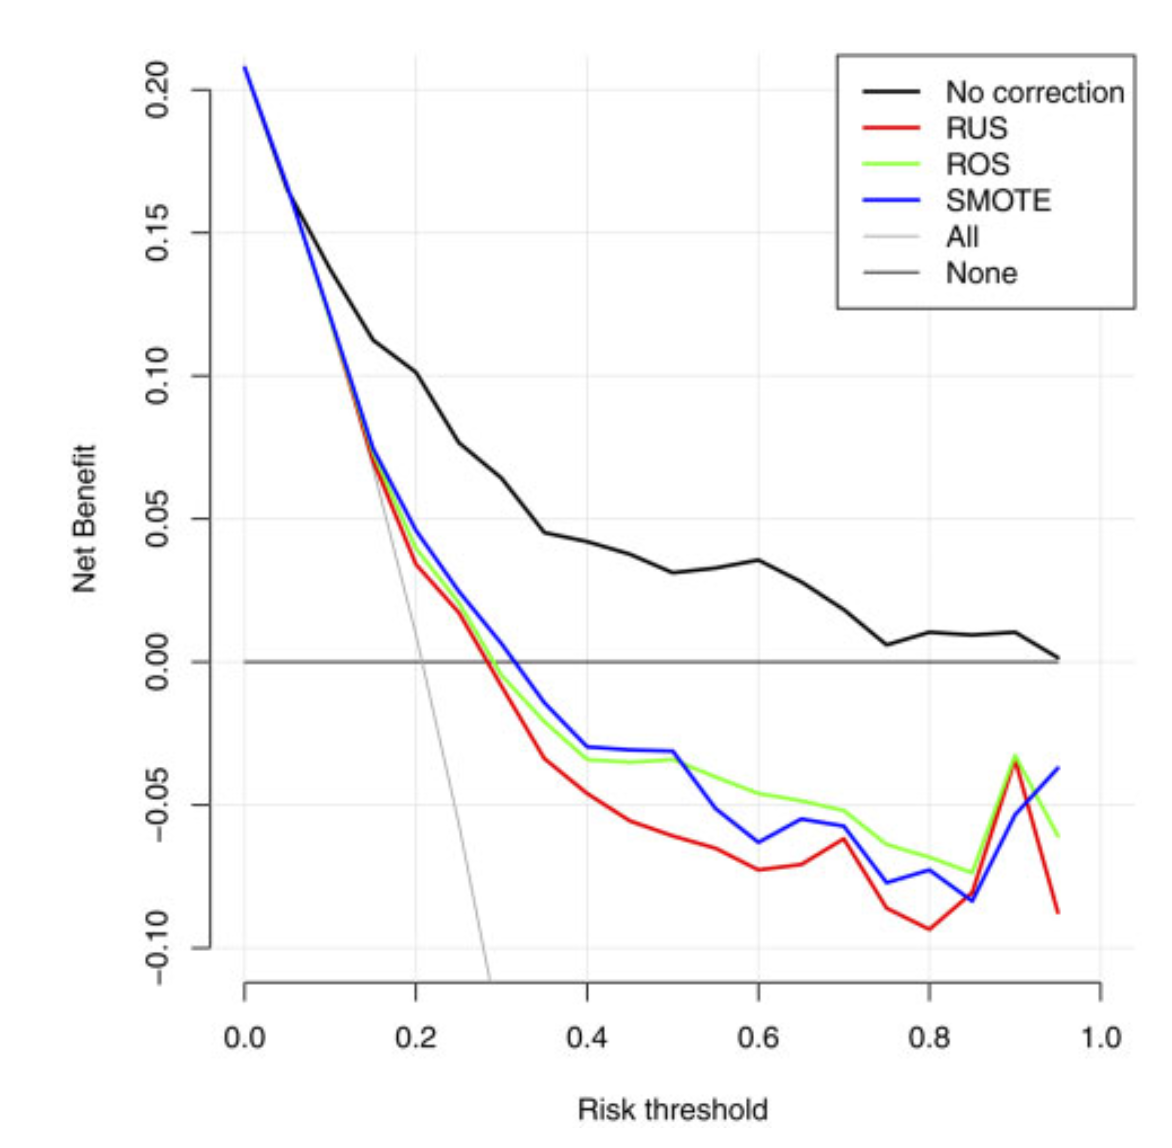
\includegraphics[height=0.5\textheight]{assets/harm_class_imbalance_corr/risk_benefit_SMOTE_RUS_ROS.png}
         	\caption{Risk vs Net Benefit for uncorrected vs ROS, RUS and SMOTE}
         \end{figure}
=======
>>>>>>> baseline
	The key finding of our work is that training logistic regression models on imbalance corrected data did not lead to better AUROC 
	compared to models trained on uncorrected data, but did result in strong and systematic overestimation of the probability for the minority class. 
	In addition, all imbalance corrections had negative consequences for the calibration slope. 
	The lower the event fraction, the more outspoken the results.
	
	Strong miscalibration reduces the clinical utility of a prediction model.30 Models yielding probability estimates that are clearly too high may lead to overtreatment. 
	For example, if a model overestimates the risk of malignancy of a detected ovarian tumor, the decision to refer patients to specialized surgery may be taken too quickly. 
	Class imbalance is often framed as problematic in the context of prediction models that classify patients into low-risk versus high-risk groups. 
	Nevertheless, for clinical prediction models the accurate estimation of probabilities is essential to help in defining such low-risk and high-risk groups. 
	For instance, clinical staff using the model to support treatment decisions may choose probability thresholds
<<<<<<< HEAD
	to match the assumed misclassification costs that best fit the context.
	
	In contrast, our study suggests that, at least for logistic regression models, 
	RUS (or ROS or SMOTE) is unlikely to lead to better discrimination or separability between the minority and majority classes.
	
\subsection{Conclusion}	
	Our study shows that correcting class imbalance did not result in better prediction models based on standard or ridge logistic regression. 
	The imbalance corrections resulted in inaccurate probability estimates without improving discrimination in terms of AUROC.
	
	
=======
	to match the assumed misclassification costs that best fit the context.
>>>>>>> baseline
